% FinalExam.tex                 25/04/07
% $Author: predrag $ $Date: 2007-05-05 15:27:24 -0400 (Sat, 05 May 2007) $
% based on /NUcourses/D60-chaos99/FinalExam.tex 04/6/99
% based on ks.tex, PC               30/6/96 

\documentclass[letterpaper,10pt,fleqn,notitlepage]{article}
\input setup
\input defs        %% the Das Buch style definitions


\title{Kuramoto-Sivashinsky turbulence:
       \\ a fishing expedition}
\author{Matt Marshall, % <raequin[snail]gmail.com>, 
        % Predrag Cvitanovi\'c, 
        {\em  et al.}
        }
%       \footnote{
% Center for Nonlinear Science,
% School of Physics, Georgia Institute of Technology,
% Atlanta, GA 30332-0430
%                     }

\date{May 6, 2007}

\begin{document}

\maketitle

 Field trip by the 
Georgia Tech PHYS 4267/7224 `Introduction to nonlinear dynamics and chaos'
class, spring semester 2007

\section{Fluttering flame front}

Turbulent flow drives a fluid through a
repertoire of unstable patterns.
As we watch a turbulent system evolve, 
every so often we catch a glimpse of a familiar pattern. 
For any finite  spatial resolution, for a finite time 
the system follows approximately
a pattern belonging to a finite 
alphabet of admissible patterns, and the long term dynamics can be thought
of as a walk through the space of such patterns,
just as chaotic dynamics with a  low dimensional
attractor can be thought of as a succession of nearly periodic (but
unstable) motions.

Here we apply this vision to
the flame flutter of gas burning 
on your kitchen stove. 
We are happy if in a few days of experimentation we succeed in simulating
the system numerically, and develop some intuition about turbulence.

\section{Problem formulation}

\noindent
Please read the chapter ``Turbulence?"\rf{DasBuch}

A flame front is
described by the Kuramoto-Sivashinsky [KS] equation
\begin{equation}
u_t= - \frac{1}{2}(u^2)_x-u_{xx}-u_{xxxx} 
\,.
\label{ks}
\end{equation}
Here $t \geq 0$ is the time and
$x \in [0,L]$ is the periodic space coordinate.
In what follows we use interchangeably the ``dimensionless
system size'' $\tildeL$, or the periodic domain size $L= 2\pi \tildeL$,
as the system parameter.
The subscripts $x$ and $t$ denote the partial derivatives with respect to 
$x$ and $t$;
$u_t = du/dt$, $u_{xxxx}$ stands for 4th spatial
derivative of the ``velocity of the flame front''
$u=u(x,t)$ at position $x$ and time $t$. 

 As the ``flame front velocity''
$u(x,t)=u(x+2\pi,t)$  is periodic on the  $x \in [0,2\pi]$ interval,
expand it in a spatial Fourier basis: 
\begin{equation}
  u(x,t)=\sum_{k=-\infty}^{+\infty} a_k (t) e^{ i k x /\tildeL }
\, . 
\label{fseries}
\end{equation}
Since $u(x,t)$ is real, 
\begin{equation}
a_k=a_{-k}^*
\,.
\label{cplx-b}
\end{equation}
Substituting (\ref{fseries}) into (\ref{ks}) yields 
the infinite ladder of evolution equations for 
the complex Fourier coefficients $a_k(t)$:
\beq
\dot{a}_k= \pVeloc_k(a)
     = ( (k/\tildeL)^2 - ( k/\tildeL)^4 )\, a_k
    - i \frac{k}{2\tildeL} \sum_{m=-\infty}^{+\infty} a_m a_{k-m}
\,.
\ee{expanfull}
As  $\dot{a}_0=0$, the  solution integrated over space is 
constant in time. We set this average velocity to 
zero, $a_0 = \int\! dx \, u(x,t) =0$.    
The coefficients $a_k$ are in general complex functions of time. 
The constant solution $u(x,t)=0$ is an
\eqv\ point of \refeq{ks}. For this ``laminar'' \eqv\ the {\stabmat}
is diagonal, 
\beq
{\Mvar}_{kj}(a) % =\frac{\pde v_k(a)}{ \pde a_j  }
=\left( {k^2}/{\tildeL^2} - {k^4}/{\tildeL^4}  \right) \delta_{kj}
\,,
\ee{expanMvar}
and
so is the {\jacobianM}
$
\jMps^t_{kj} = \delta_{kj} e^{(k/\tildeL)^2(1- (k/\tildeL)^2)t}
\,.
$
From 
(\ref{expanMvar}) it follows that the $|k|< \tildeL$ 
long wavelength modes of this 
\eqv\ are linearly unstable, and the 
$|k|>\tildeL$ short wavelength modes are stable.  
For $\tildeL < 1$,  $u(x,t)=0$ is the globally attractive stable \eqv,
{\em i.e.}, the dissipation is so strong that any flame front burns out.


\subsection{Energy budget}

A theory of turbulence  should
predict measurable properties of turbulent flows, such as
their mean energies and their energy dissipation rates.


The time-dependent average velocity-squared
\beq
    E =\frac{1}{L}\int_0^{L}\! dx \, \frac{u^2}{2}
\label{ksEnergy}
\eeq
has a physical interpretation
as the average ``kinetic energy'' density of the flame front.
Its time evolution is given by the power/dissipation energy rate equation
\beq
   \dot{E} = P - D
                \,,\qquad
      P =  \expct{(u_{x})^2}
                \,,\quad
      D =  \expct{(u_{xx})^2}
.
\ee{EnRate}
KS is a far-from equilibrium system:  
the power $P$
pumped in by the anti-diffusion $u_{xx}$
is
balanced by the hypervicosity $u_{xxxx}$ 
dissipation rate $D$. In principle,
these are experimentally observable quantities, 
used 
in what follows as flow diagnostics.

\subsection{Computation}

We used R.~L.~Davidchack's implementation of Kassam and Trefethen code\cite{ks04com}:

{\tt ChaosBook.org/extras/\#PDEs} .

\section{Fishing}

From here on we turn to numerical experimentation.
Take $L$ sufficiently large so that the
dynamics can be spatiotemporally chaotic, but not so large that we would be
overwhelmed by many short wavelength modes needed in order to accurately
represent the dynamics.

A bit of advice: start on {\em terra firma}, 
small system size  $\tildeL = 1$, 
%low truncation $N$, 
and increase  $\tildeL$ a little bit, integrate until the
trajectory has settled down; then increase  $\tildeL$ a little bit again,
restart from the trajectory just computed, 
integrate until has settled down. 
Repeat. Sometimes stop incrementing
the trajectory, increment $N$ instead and check how sensitive is your
attractor to truncation number $N$. This ``adiabatic''
approach has advantage of (almost) always starting you close to
the attractor, thus avoiding long transients typical of random
starting conditions.

The problem with high-dimensional truncations of (\ref{expanfull})
is that the dynamics is difficult to visualize. 
We visualize a trajectory by its projections onto any three 
2 or 3 basis vectors (states of the system):
see Davidchack code for  examples.



%%%%%%%%%%%%%%%%%%%%%%%%%%%%%%%%%%%%%%%%%%%%%%%%%%%%%%%%%%%%%%%%
\begin{figure}[t]       \label{fig:GreeneKim}
\begin{center}
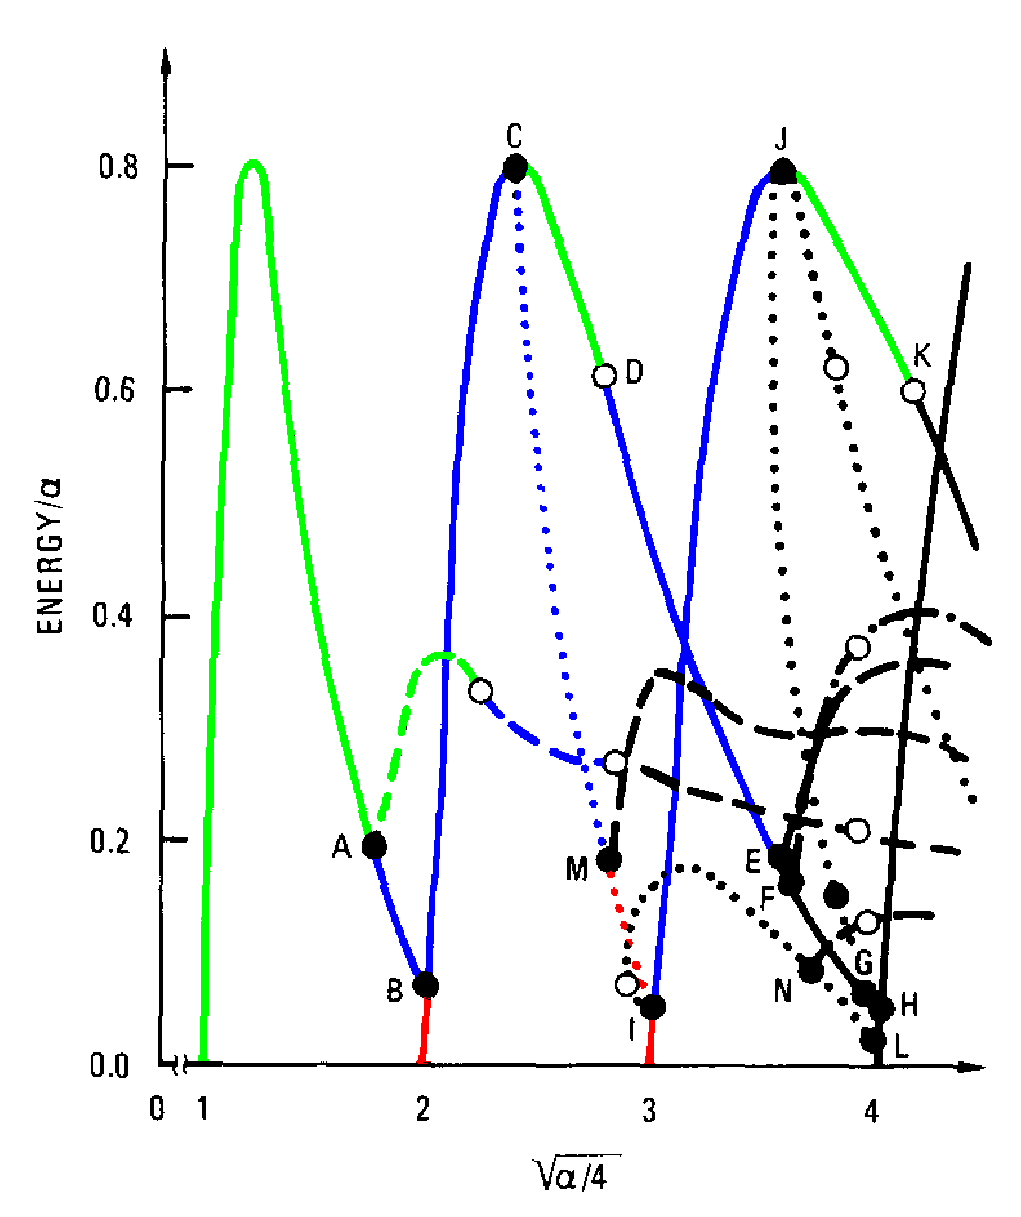
\includegraphics[width=0.5\textwidth]{GreeneKimBifColor.eps}
\end{center}
\caption{
The energy \refeq{ksEnergy}  of all  \eqva\ that exist up 
to $\tildeL = 4.5$
plotted as a function of the system size
$\tildeL$ (from \refref{ksgreene88}).
Solid curves denote $n$-cell solutions,
dotted curves GLMRT, the dash-dotted curve the
`giant states', and dashed curves the \reqva.
Open circles indicate Hopf bifurcations.
The color of a branch indicates the number of unstable
eigenvalues: (red) 2 unstable eigenvalues, (blue) 1
unstable eigenvalue, (green) stable.
        }
\end{figure}
%%%%%%%%%%%%%%%%%%%%%%%%%%%%%%%%%%%%%%%%%%%%%%%%%%%%%%%%%%%%%%%%%%

\subsection{Bifurcations with the  increase of system size $L$}

Explore dynamics for different system sizes $L$
by plotting long trajectories both in the \statesp\ and
in color-coded space-time plots of $u(x,t)$. If the long
time trajectory is settling on an
attractive \eqv\ or \po, eliminate the initial
transient by starting the plots only after the
transients have died out.

Classical papers on the \eqva\ of
\KSe, bifurcations and symmetry analysis are
Kevrekidis, Nicolaenko and Scovel\rf{KNSks90},
and Greene and Kim\rf{ksgreene88}. You might be able to 
identify your states in the 
\reffig{fig:GreeneKim} bifurcation diagram.
To get the right $E$, multiply
by 4; the horizontal axis is $\tildeL = \sqrt{\alpha/4}$.
  


Here is what the class fished out, listed as
series of numerical experiments ordered by $\tildeL$ parameter.
Please send you .png files to 
Matt Marshall, {\tt raequin[snail]gmail.com}

\begin{itemize}
\item[1.5915494:] $L = 10$ (Holt)
        \\stable \EQV{1}
\item[1.7603981:] $\tildeL = 1+\pi/4-0.025$ (Marshall)
       \\        
        What's this bifurcation? Narrow the gap $\pm 0.025$
        to see whether it really happens at
        $\tildeL = 1+\pi/4 \pm \epsilon$. Why would that happen?
\item[1.8103981:] $\tildeL = 1+\pi/4+0.025$ (Marshall)
       \\
\item[1.9098593:] $L = 12$ (Holt, Hermand)
        \\stable periodic orbit
\item[2:] $\tildeL = 2$ (Marshall)
       \\
\item[2.0690142:] $L = 13$ (Iacobucci)
       \\ relative periodic?
\item[2.078125:]  $ \tildeL = 2+5/64$ (Marshall)
       \\ slowly drifting relative periodic?
\item[2.09375:] $ \tildeL = 2+3/32$ (Marshall)
       \\ flipping between \EQV{1} and 1/2 shifted \EQV{1}?
\item[2.1591549:] $\tildeL = 2+1/2\pi$ (Marshall)
       \\ flipping between \EQV{1} and 1/2 shifted \EQV{1}?
\item[2.2281692:] $L = 14$ (Hermand)
        \\ stable \EQV{2}
\\item[2.5:] $ \tildeL = 2+1/2$ (Marshall)
       \\why does this trajectory project to $(0,0,0)$ 
    in Ruslan's $(v_1,v_2,v_3)$ basis?
\item[2.8647882:] $L = 18$ (Marshall, Hermand)
       \\ attractive cycle?
\item[3:] $L = 3$ (Sonenblum)
       \\ flipping between \EQV{1} and 1/2 shifted \EQV{1}?
\item[3.0239439:] $L = 19$ (Holt)
        \\stable \EQV{2}
\item[3.22:] $ \tildeL = 2.5+3/4-0.03$ (Marshall)
       \\ attractive cycle
\item[3.28:] $ \tildeL = 2.5+3/4+0.03$ (Marshall)
       \\ flipping between \EQV{2} and 1/2 shifted \EQV{2},
        via the above unstable cycle neighborhood?
        What's this bifurcation? Narrow the gap $\pm 0.03$
        to see whether it really happens at
        $ \tildeL = 2.5+3/4 \pm \epsilon$
\item[3.3422538:] $L = 21$ (Li)
        \\ relative periodic attractor? unclear
\item[3.6605636:] $L = 23$ (Davydychev, Holt)
        \\ strange - looks like cycle but keeps flipping
\item[3.8197186:] $L = 24$ (Hermand, Silverman)
        \\ spiral into \EQV{3} attractor
\item[3.8408862:] $L = 24.133$ (Marshall)
        \\ spiral into \EQV{3} attractor
\item[3.978873:] $L = 25$ (Li, Hermand)
        \\ spiral into \EQV{3} attractor
\item[4.138028:] $L = 26$ (Anzalone, Iacobucci, Holt)
        \\ unclear. Iacobucci drifting 3-cycle,  Holt 3-cycle
\item[4.4563384:] $L = 28$ (Davydychev)
        \\equilibrium
\item[4.6154933:] $L = 29$ (Hermand)
        \\settles into a wierd state, asymptotic only after $t>250$
\item[5:] $L = 5$ (Sonenblum)
        \\ stable \EQV{4}
\item[5.411268:] $L = 34$ (Freeman)
       \\ co-existing attractors?
\item[6.3661977:] $L = 40$ (Iacobucci)
       \\ interesting transient
\item[7:] $L = 7$ (Sonenblum)
        \\ turbulent
\item[9:] $L = 9$ (Sonenblum)
        \\ turbulent


\end{itemize}

\subsection{Energy dependence on $L$}

Iacobucco and Freeman have interesting ways of scanning 
energy as function of $L$.
With this they have explored bifurcation sequences 
by plotting ({\em inter alia}) the time-averaged values 
$(\timeAver{E},\timeAver{P},\timeAver{D})$ of $(E,P,D)$ 
defined in \refeq{EnRate}, for small increments of
$ 1< L < 25$.

\subsection{Turbulence at $\tildeL=22$?}

\begin{enumerate}
\item
{\bf Plot} several long trajectories for  $L = 22$,
different initial conditions, 
using the same vector basis as Davidchack. Is your dynamics
qualitatively the same as in his plots?

[Holt has nice long time runs]

\item
Do you get any stable periodic orbits for $\tildeL=22$? 
If you do, we would love to see them - have not found any.

[Nobody saw anything different, and no stable orbits
were observed. Only Sharon tried a set of different initial conditions,
but al close-by]
\end{enumerate}


\section{Turbulence goes Hollywood}

Kirill Davydychev:  % <russian[snail]gatech.edu> 
I left my laptop overnight to compute this
flame front  movie:

\href{FlameFrontKD.avi}{FlameFront [avi format]}.

From it 
one can guess the stable/unstable cycles, the
period for them seems to be around $7L$, with $3.5 \, L$ separation.
\PC{you mean period in time, or that by increasing \tildeL\ by
    1 you see another bifurcation?
    }

Also, here is a geeky approach to the onset of chaos:
consider the file
sizes of each frame. In a lossless format such as .png, the
compression ratio is an indicator of the complexity of the
structure, see \href{KDfileCompress.png}{graph of $L$ vs. the file size}. 
It correlates with the chaotic behavior of this system
(not to mention that it's also completely useless).


Now, have a Carlsberg, perhaps the best beer 
in some parts of Copenhagen, and a good summer.

\bibliographystyle{unsrt}
\bibliography{course}

\end{document}  
